\documentclass[aspectratio=169,11pt]{beamer}
% =====================================================================
%  pds-beamer.tex — Estilo común de las transparencias.
%
%  Uso (desde teoría/Tx/transparencias/):
%     \documentclass[aspectratio=169,11pt]{beamer}
%     % =====================================================================
%  pds-beamer.tex — Estilo común de las transparencias.
%
%  Uso (desde teoría/Tx/transparencias/):
%     \documentclass[aspectratio=169,11pt]{beamer}
%     % =====================================================================
%  pds-beamer.tex — Estilo común de las transparencias.
%
%  Uso (desde teoría/Tx/transparencias/):
%     \documentclass[aspectratio=169,11pt]{beamer}
%     \input{../../comun/pds-beamer}
%     \title{...}  \subtitle{Tema x · ...}
%     \begin{document}
%       \portada
%       ...
%     \end{document}
%  Compilar con:  latexmk -xelatex  (o «make» desde teoría/)
% =====================================================================

\usetheme{Boadilla}
\usecolortheme{orchid}
\usefonttheme{professionalfonts}
\setbeamercovered{transparent}
\setbeamersize{text margin left=0.8cm, text margin right=0.8cm}
\setbeamertemplate{navigation symbols}{}
\setbeamertemplate{itemize item}[square]
\setbeamertemplate{itemize subitem}[circle]
\setbeamertemplate{itemize subsubitem}[triangle]
\setbeamertemplate{enumerate item}[square]
\setbeamertemplate{enumerate subitem}[circle]
\setbeamertemplate{caption}{\raggedright\insertcaption\par}

\input{../../comun/pds-comun.tex}

% Tipografía: Fira Sans + Fira Math (legibles en proyector)
\usepackage{fontspec}
\usepackage{unicode-math}
% Se cargan por nombre de fichero para que funcionen con cualquier
% instalación de TeX Live (o MiKTeX) sin instalar fuentes en el sistema.
\setmainfont{FiraSans}[Extension=.otf, UprightFont=*-Regular, BoldFont=*-SemiBold,
  ItalicFont=*-Italic, BoldItalicFont=*-SemiBoldItalic]
\setsansfont{FiraSans}[Extension=.otf, UprightFont=*-Regular, BoldFont=*-SemiBold,
  ItalicFont=*-Italic, BoldItalicFont=*-SemiBoldItalic]
\setmonofont{FiraMono}[Extension=.otf, UprightFont=*-Regular, BoldFont=*-Medium, AutoFakeSlant=0.15, Scale=0.92]
\setmathfont{FiraMath-Regular.otf}
\setmathfont{latinmodern-math.otf}[range={"229B,"22EE,"22F1}]

% Colores del tema ajustados a la paleta común (más contraste)
\setbeamercolor{structure}{fg=pdsazul}
\setbeamercolor{alerted text}{fg=pdsrojo}
\setbeamercolor{example text}{fg=pdsverde}
\setbeamercolor{block title}{bg=pdsazul, fg=white}
\setbeamercolor{block body}{bg=pdsfondo}
\setbeamercolor{block title alerted}{bg=pdsrojo, fg=white}
\setbeamercolor{block body alerted}{bg=pdsrojo!6}
\setbeamercolor{block title example}{bg=pdsverde, fg=white}
\setbeamercolor{block body example}{bg=pdsverde!6}
\setbeamercolor{frametitle}{fg=pdsazul, bg=white}
\setbeamerfont{frametitle}{size=\large, series=\bfseries}
\setbeamerfont{block title}{size=\normalsize, series=\bfseries}
\setbeamertemplate{blocks}[rounded][shadow=false]

% Logo en la esquina superior derecha de cada transparencia
\pgfdeclareimage[height=0.8cm]{logo}{../../comun/ucm.png}
\addtobeamertemplate{frametitle}{}{%
  \begin{tikzpicture}[remember picture, overlay]
    \node[anchor=north east, inner sep=0pt] at ([xshift=-0.25cm, yshift=-0.2cm]current page.north east) {\pgfuseimage{logo}};
  \end{tikzpicture}}

% Datos de portada
\author[\autorescorto]{\autores}
\institute[UCM]{\footnotesize\departamento\\\universidad}
\date[\curso]{\footnotesize\grado\\\curso}

\newcommand{\portada}{%
  \begin{frame}[plain]
    \begin{center}
      
\includegraphics[height=1.9cm]{../../comun/ucm.png}
    \end{center}
    \vspace{-0.4cm}
    \titlepage
  \end{frame}}

% Índice al empezar cada sección
\AtBeginSection[]{%
  \begin{frame}{Contenido}
    \tableofcontents[currentsection, hideothersubsections]
  \end{frame}}

\renewcommand{\pdscodesize}{\scriptsize}

% Utilidades
% \herramienta{T1-convolucion-continua}: enlace a la página publicada de
% herramientas/html (se abre en el navegador, sin instalar nada).
% \herramientaservidor{server/....py}: app que necesita Python (bokeh serve).
\newcommand{\urlherramientas}{https://ucm-237.github.io/PdS/}
\newcommand{\herramienta}[1]{%
  \par\vfill\hfill{\scriptsize\color{pdsgris}\faIcon\ \href{\urlherramientas#1.html}{Herramienta interactiva: \texttt{#1}}}}
\newcommand{\herramientaservidor}[1]{%
  \par\vfill\hfill{\scriptsize\color{pdsgris}\faIcon\ Herramienta interactiva (con Python): \texttt{herramientas/#1}}}
\newcommand{\faIcon}{\textbf{▶}}
\newcommand{\gris}[1]{{\color{pdsgris}#1}}
\newcommand{\nota}[1]{\par\vspace{2pt}{\footnotesize\color{pdsgris}\textit{#1}}\par}
% Nota sobre una errata de versiones anteriores (solo con \ERRATAS)
\newcommand{\errata}[1]{\iferratas\nota{Errata de versiones anteriores: #1}\fi}
\newcommand{\apuntes}[1]{\nota{Más detalle en los apuntes, #1.}}

% Bloques con nombre en castellano
\newenvironment{definicion}[1][Definición]{\begin{block}{#1}}{\end{block}}
\newenvironment{importante}[1][Importante]{\begin{alertblock}{#1}}{\end{alertblock}}
\newenvironment{ejemplo}[1][Ejemplo]{\begin{exampleblock}{#1}}{\end{exampleblock}}

%     \title{...}  \subtitle{Tema x · ...}
%     \begin{document}
%       \portada
%       ...
%     \end{document}
%  Compilar con:  latexmk -xelatex  (o «make» desde teoría/)
% =====================================================================

\usetheme{Boadilla}
\usecolortheme{orchid}
\usefonttheme{professionalfonts}
\setbeamercovered{transparent}
\setbeamersize{text margin left=0.8cm, text margin right=0.8cm}
\setbeamertemplate{navigation symbols}{}
\setbeamertemplate{itemize item}[square]
\setbeamertemplate{itemize subitem}[circle]
\setbeamertemplate{itemize subsubitem}[triangle]
\setbeamertemplate{enumerate item}[square]
\setbeamertemplate{enumerate subitem}[circle]
\setbeamertemplate{caption}{\raggedright\insertcaption\par}

% =====================================================================
%  pds-comun.tex — Paquetes, colores y estilos de código comunes a
%  transparencias, apuntes y hojas de ejercicios. Compilar con XeLaTeX.
%  No cargar directamente: lo cargan pds-beamer.tex y pds-apuntes.tex.
% =====================================================================

\usepackage{polyglossia}
\setmainlanguage{spanish}
\usepackage{mathtools}
\usepackage{graphicx}
\usepackage{booktabs}
\usepackage{multirow}
\usepackage{array}
\usepackage{xcolor}
\usepackage{tikz}
\usetikzlibrary{positioning,arrows.meta,calc,shapes.geometric,decorations.pathreplacing}
\usepackage{listings}
\usepackage{siunitx}
\sisetup{output-decimal-marker={,}, group-separator={\,}, per-mode=symbol}

% Notas de erratas de versiones anteriores: no se imprimen salvo que se
% defina \ERRATAS antes de cargar el estilo (make ERRATAS=1)
\newif\iferratas
\ifdefined\ERRATAS \erratastrue \fi

% Ruta común (logo y figuras compartidas)
\providecommand{\rutacomun}{../../comun/}
\input{\rutacomun datos.tex}

% ---------------------------------------------------------------------
%  Paleta (la misma que usan las figuras generadas con Python,
%  ver comun/pds_estilo.py)
% ---------------------------------------------------------------------
\definecolor{pdsazul}{HTML}{2B3A8C}
\definecolor{pdsrojo}{HTML}{C0392B}
\definecolor{pdsverde}{HTML}{1E7B4F}
\definecolor{pdsnaranja}{HTML}{D9822B}
\definecolor{pdsgris}{HTML}{5A5A66}
\definecolor{pdsfondo}{HTML}{F3F4FA}
\definecolor{pdscodigo}{HTML}{F7F7F2}

% ---------------------------------------------------------------------
%  Diagramas de bloques (TikZ)
% ---------------------------------------------------------------------
\tikzset{
  bloque/.style={rectangle, rounded corners=2pt, draw=pdsazul!80, fill=pdsfondo,
                 very thick, minimum height=8mm, minimum width=14mm, align=center},
  sumador/.style={circle, draw=pdsazul!80, fill=pdsfondo, thick, inner sep=1.5pt},
  flecha/.style={-{Stealth[length=2.2mm]}, thick, pdsgris},
}

% ---------------------------------------------------------------------
%  Código: Python y Matlab en paralelo
% ---------------------------------------------------------------------
\newcommand{\pdscodesize}{\footnotesize}
\lstdefinestyle{pds}{
  basicstyle=\ttfamily\pdscodesize,
  keywordstyle=\color{pdsazul}\bfseries,
  commentstyle=\color{pdsverde}\itshape,
  stringstyle=\color{pdsrojo},
  numbers=none,
  backgroundcolor=\color{pdscodigo},
  frame=single, rulecolor=\color{pdsgris!40}, framerule=0.4pt,
  xleftmargin=2pt, xrightmargin=2pt, aboveskip=2pt, belowskip=2pt,
  columns=fullflexible, keepspaces=true,
  showstringspaces=false, breaklines=true, tabsize=4,
  upquote=true,
  % Con XeLaTeX, listings desordena los caracteres no ASCII junto a
  % dígitos («2π» sale «π2»): se sustituyen por su versión matemática.
  literate={π}{{$\pi$}}1 {δ}{{$\delta$}}1 {ω}{{$\omega$}}1 {Ω}{{$\Omega$}}1
           {≈}{{$\approx$}}1 {µ}{{$\mu$}}1 {·}{{$\cdot$}}1 {α}{{$\alpha$}}1
           {á}{{á}}1 {é}{{é}}1 {í}{{í}}1 {ó}{{ó}}1 {ú}{{ú}}1 {ñ}{{ñ}}1 {¿}{{¿}}1,
}
\lstdefinestyle{python}{style=pds, language=Python,
  morekeywords={as,True,False,None}}
\lstdefinestyle{matlab}{style=pds, language=Matlab,
  morekeywords={function,end,true,false}}

% \codigo{<ruta sin extensión>} muestra el mismo ejemplo en Python
% y en Matlab, uno al lado del otro. Los ficheros viven en
% ../codigo/python/<nombre>.py y ../codigo/matlab/<nombre>.m y se
% ejecutan en las pruebas (make prueba-codigo).
\newcommand{\rutacodigo}{../codigo/}
\newcommand{\codigoetiqueta}[1]{{\sffamily\scriptsize\bfseries\color{pdsgris}#1}}
\newcommand{\codigo}[2][]{%
  \par\noindent
  \begin{minipage}[t]{0.495\linewidth}
    \codigoetiqueta{Python}\par\vspace{1pt}
    \lstinputlisting[style=python,#1]{\rutacodigo python/#2.py}
  \end{minipage}\hfill
  \begin{minipage}[t]{0.495\linewidth}
    \codigoetiqueta{Matlab}\par\vspace{1pt}
    \lstinputlisting[style=matlab,#1]{\rutacodigo matlab/#2.m}
  \end{minipage}\par}

\input{\rutacomun notacion.tex}


% Tipografía: Fira Sans + Fira Math (legibles en proyector)
\usepackage{fontspec}
\usepackage{unicode-math}
% Se cargan por nombre de fichero para que funcionen con cualquier
% instalación de TeX Live (o MiKTeX) sin instalar fuentes en el sistema.
\setmainfont{FiraSans}[Extension=.otf, UprightFont=*-Regular, BoldFont=*-SemiBold,
  ItalicFont=*-Italic, BoldItalicFont=*-SemiBoldItalic]
\setsansfont{FiraSans}[Extension=.otf, UprightFont=*-Regular, BoldFont=*-SemiBold,
  ItalicFont=*-Italic, BoldItalicFont=*-SemiBoldItalic]
\setmonofont{FiraMono}[Extension=.otf, UprightFont=*-Regular, BoldFont=*-Medium, AutoFakeSlant=0.15, Scale=0.92]
\setmathfont{FiraMath-Regular.otf}
\setmathfont{latinmodern-math.otf}[range={"229B,"22EE,"22F1}]

% Colores del tema ajustados a la paleta común (más contraste)
\setbeamercolor{structure}{fg=pdsazul}
\setbeamercolor{alerted text}{fg=pdsrojo}
\setbeamercolor{example text}{fg=pdsverde}
\setbeamercolor{block title}{bg=pdsazul, fg=white}
\setbeamercolor{block body}{bg=pdsfondo}
\setbeamercolor{block title alerted}{bg=pdsrojo, fg=white}
\setbeamercolor{block body alerted}{bg=pdsrojo!6}
\setbeamercolor{block title example}{bg=pdsverde, fg=white}
\setbeamercolor{block body example}{bg=pdsverde!6}
\setbeamercolor{frametitle}{fg=pdsazul, bg=white}
\setbeamerfont{frametitle}{size=\large, series=\bfseries}
\setbeamerfont{block title}{size=\normalsize, series=\bfseries}
\setbeamertemplate{blocks}[rounded][shadow=false]

% Logo en la esquina superior derecha de cada transparencia
\pgfdeclareimage[height=0.8cm]{logo}{../../comun/ucm.png}
\addtobeamertemplate{frametitle}{}{%
  \begin{tikzpicture}[remember picture, overlay]
    \node[anchor=north east, inner sep=0pt] at ([xshift=-0.25cm, yshift=-0.2cm]current page.north east) {\pgfuseimage{logo}};
  \end{tikzpicture}}

% Datos de portada
\author[\autorescorto]{\autores}
\institute[UCM]{\footnotesize\departamento\\\universidad}
\date[\curso]{\footnotesize\grado\\\curso}

\newcommand{\portada}{%
  \begin{frame}[plain]
    \begin{center}
      
\includegraphics[height=1.9cm]{../../comun/ucm.png}
    \end{center}
    \vspace{-0.4cm}
    \titlepage
  \end{frame}}

% Índice al empezar cada sección
\AtBeginSection[]{%
  \begin{frame}{Contenido}
    \tableofcontents[currentsection, hideothersubsections]
  \end{frame}}

\renewcommand{\pdscodesize}{\scriptsize}

% Utilidades
% \herramienta{T1-convolucion-continua}: enlace a la página publicada de
% herramientas/html (se abre en el navegador, sin instalar nada).
% \herramientaservidor{server/....py}: app que necesita Python (bokeh serve).
\newcommand{\urlherramientas}{https://ucm-237.github.io/PdS/}
\newcommand{\herramienta}[1]{%
  \par\vfill\hfill{\scriptsize\color{pdsgris}\faIcon\ \href{\urlherramientas#1.html}{Herramienta interactiva: \texttt{#1}}}}
\newcommand{\herramientaservidor}[1]{%
  \par\vfill\hfill{\scriptsize\color{pdsgris}\faIcon\ Herramienta interactiva (con Python): \texttt{herramientas/#1}}}
\newcommand{\faIcon}{\textbf{▶}}
\newcommand{\gris}[1]{{\color{pdsgris}#1}}
\newcommand{\nota}[1]{\par\vspace{2pt}{\footnotesize\color{pdsgris}\textit{#1}}\par}
% Nota sobre una errata de versiones anteriores (solo con \ERRATAS)
\newcommand{\errata}[1]{\iferratas\nota{Errata de versiones anteriores: #1}\fi}
\newcommand{\apuntes}[1]{\nota{Más detalle en los apuntes, #1.}}

% Bloques con nombre en castellano
\newenvironment{definicion}[1][Definición]{\begin{block}{#1}}{\end{block}}
\newenvironment{importante}[1][Importante]{\begin{alertblock}{#1}}{\end{alertblock}}
\newenvironment{ejemplo}[1][Ejemplo]{\begin{exampleblock}{#1}}{\end{exampleblock}}

%     \title{...}  \subtitle{Tema x · ...}
%     \begin{document}
%       \portada
%       ...
%     \end{document}
%  Compilar con:  latexmk -xelatex  (o «make» desde teoría/)
% =====================================================================

\usetheme{Boadilla}
\usecolortheme{orchid}
\usefonttheme{professionalfonts}
\setbeamercovered{transparent}
\setbeamersize{text margin left=0.8cm, text margin right=0.8cm}
\setbeamertemplate{navigation symbols}{}
\setbeamertemplate{itemize item}[square]
\setbeamertemplate{itemize subitem}[circle]
\setbeamertemplate{itemize subsubitem}[triangle]
\setbeamertemplate{enumerate item}[square]
\setbeamertemplate{enumerate subitem}[circle]
\setbeamertemplate{caption}{\raggedright\insertcaption\par}

% =====================================================================
%  pds-comun.tex — Paquetes, colores y estilos de código comunes a
%  transparencias, apuntes y hojas de ejercicios. Compilar con XeLaTeX.
%  No cargar directamente: lo cargan pds-beamer.tex y pds-apuntes.tex.
% =====================================================================

\usepackage{polyglossia}
\setmainlanguage{spanish}
\usepackage{mathtools}
\usepackage{graphicx}
\usepackage{booktabs}
\usepackage{multirow}
\usepackage{array}
\usepackage{xcolor}
\usepackage{tikz}
\usetikzlibrary{positioning,arrows.meta,calc,shapes.geometric,decorations.pathreplacing}
\usepackage{listings}
\usepackage{siunitx}
\sisetup{output-decimal-marker={,}, group-separator={\,}, per-mode=symbol}

% Notas de erratas de versiones anteriores: no se imprimen salvo que se
% defina \ERRATAS antes de cargar el estilo (make ERRATAS=1)
\newif\iferratas
\ifdefined\ERRATAS \erratastrue \fi

% Ruta común (logo y figuras compartidas)
\providecommand{\rutacomun}{../../comun/}
\input{\rutacomun datos.tex}

% ---------------------------------------------------------------------
%  Paleta (la misma que usan las figuras generadas con Python,
%  ver comun/pds_estilo.py)
% ---------------------------------------------------------------------
\definecolor{pdsazul}{HTML}{2B3A8C}
\definecolor{pdsrojo}{HTML}{C0392B}
\definecolor{pdsverde}{HTML}{1E7B4F}
\definecolor{pdsnaranja}{HTML}{D9822B}
\definecolor{pdsgris}{HTML}{5A5A66}
\definecolor{pdsfondo}{HTML}{F3F4FA}
\definecolor{pdscodigo}{HTML}{F7F7F2}

% ---------------------------------------------------------------------
%  Diagramas de bloques (TikZ)
% ---------------------------------------------------------------------
\tikzset{
  bloque/.style={rectangle, rounded corners=2pt, draw=pdsazul!80, fill=pdsfondo,
                 very thick, minimum height=8mm, minimum width=14mm, align=center},
  sumador/.style={circle, draw=pdsazul!80, fill=pdsfondo, thick, inner sep=1.5pt},
  flecha/.style={-{Stealth[length=2.2mm]}, thick, pdsgris},
}

% ---------------------------------------------------------------------
%  Código: Python y Matlab en paralelo
% ---------------------------------------------------------------------
\newcommand{\pdscodesize}{\footnotesize}
\lstdefinestyle{pds}{
  basicstyle=\ttfamily\pdscodesize,
  keywordstyle=\color{pdsazul}\bfseries,
  commentstyle=\color{pdsverde}\itshape,
  stringstyle=\color{pdsrojo},
  numbers=none,
  backgroundcolor=\color{pdscodigo},
  frame=single, rulecolor=\color{pdsgris!40}, framerule=0.4pt,
  xleftmargin=2pt, xrightmargin=2pt, aboveskip=2pt, belowskip=2pt,
  columns=fullflexible, keepspaces=true,
  showstringspaces=false, breaklines=true, tabsize=4,
  upquote=true,
  % Con XeLaTeX, listings desordena los caracteres no ASCII junto a
  % dígitos («2π» sale «π2»): se sustituyen por su versión matemática.
  literate={π}{{$\pi$}}1 {δ}{{$\delta$}}1 {ω}{{$\omega$}}1 {Ω}{{$\Omega$}}1
           {≈}{{$\approx$}}1 {µ}{{$\mu$}}1 {·}{{$\cdot$}}1 {α}{{$\alpha$}}1
           {á}{{á}}1 {é}{{é}}1 {í}{{í}}1 {ó}{{ó}}1 {ú}{{ú}}1 {ñ}{{ñ}}1 {¿}{{¿}}1,
}
\lstdefinestyle{python}{style=pds, language=Python,
  morekeywords={as,True,False,None}}
\lstdefinestyle{matlab}{style=pds, language=Matlab,
  morekeywords={function,end,true,false}}

% \codigo{<ruta sin extensión>} muestra el mismo ejemplo en Python
% y en Matlab, uno al lado del otro. Los ficheros viven en
% ../codigo/python/<nombre>.py y ../codigo/matlab/<nombre>.m y se
% ejecutan en las pruebas (make prueba-codigo).
\newcommand{\rutacodigo}{../codigo/}
\newcommand{\codigoetiqueta}[1]{{\sffamily\scriptsize\bfseries\color{pdsgris}#1}}
\newcommand{\codigo}[2][]{%
  \par\noindent
  \begin{minipage}[t]{0.495\linewidth}
    \codigoetiqueta{Python}\par\vspace{1pt}
    \lstinputlisting[style=python,#1]{\rutacodigo python/#2.py}
  \end{minipage}\hfill
  \begin{minipage}[t]{0.495\linewidth}
    \codigoetiqueta{Matlab}\par\vspace{1pt}
    \lstinputlisting[style=matlab,#1]{\rutacodigo matlab/#2.m}
  \end{minipage}\par}

\input{\rutacomun notacion.tex}


% Tipografía: Fira Sans + Fira Math (legibles en proyector)
\usepackage{fontspec}
\usepackage{unicode-math}
% Se cargan por nombre de fichero para que funcionen con cualquier
% instalación de TeX Live (o MiKTeX) sin instalar fuentes en el sistema.
\setmainfont{FiraSans}[Extension=.otf, UprightFont=*-Regular, BoldFont=*-SemiBold,
  ItalicFont=*-Italic, BoldItalicFont=*-SemiBoldItalic]
\setsansfont{FiraSans}[Extension=.otf, UprightFont=*-Regular, BoldFont=*-SemiBold,
  ItalicFont=*-Italic, BoldItalicFont=*-SemiBoldItalic]
\setmonofont{FiraMono}[Extension=.otf, UprightFont=*-Regular, BoldFont=*-Medium, AutoFakeSlant=0.15, Scale=0.92]
\setmathfont{FiraMath-Regular.otf}
\setmathfont{latinmodern-math.otf}[range={"229B,"22EE,"22F1}]

% Colores del tema ajustados a la paleta común (más contraste)
\setbeamercolor{structure}{fg=pdsazul}
\setbeamercolor{alerted text}{fg=pdsrojo}
\setbeamercolor{example text}{fg=pdsverde}
\setbeamercolor{block title}{bg=pdsazul, fg=white}
\setbeamercolor{block body}{bg=pdsfondo}
\setbeamercolor{block title alerted}{bg=pdsrojo, fg=white}
\setbeamercolor{block body alerted}{bg=pdsrojo!6}
\setbeamercolor{block title example}{bg=pdsverde, fg=white}
\setbeamercolor{block body example}{bg=pdsverde!6}
\setbeamercolor{frametitle}{fg=pdsazul, bg=white}
\setbeamerfont{frametitle}{size=\large, series=\bfseries}
\setbeamerfont{block title}{size=\normalsize, series=\bfseries}
\setbeamertemplate{blocks}[rounded][shadow=false]

% Logo en la esquina superior derecha de cada transparencia
\pgfdeclareimage[height=0.8cm]{logo}{../../comun/ucm.png}
\addtobeamertemplate{frametitle}{}{%
  \begin{tikzpicture}[remember picture, overlay]
    \node[anchor=north east, inner sep=0pt] at ([xshift=-0.25cm, yshift=-0.2cm]current page.north east) {\pgfuseimage{logo}};
  \end{tikzpicture}}

% Datos de portada
\author[\autorescorto]{\autores}
\institute[UCM]{\footnotesize\departamento\\\universidad}
\date[\curso]{\footnotesize\grado\\\curso}

\newcommand{\portada}{%
  \begin{frame}[plain]
    \begin{center}
      
\includegraphics[height=1.9cm]{../../comun/ucm.png}
    \end{center}
    \vspace{-0.4cm}
    \titlepage
  \end{frame}}

% Índice al empezar cada sección
\AtBeginSection[]{%
  \begin{frame}{Contenido}
    \tableofcontents[currentsection, hideothersubsections]
  \end{frame}}

\renewcommand{\pdscodesize}{\scriptsize}

% Utilidades
% \herramienta{T1-convolucion-continua}: enlace a la página publicada de
% herramientas/html (se abre en el navegador, sin instalar nada).
% \herramientaservidor{server/....py}: app que necesita Python (bokeh serve).
\newcommand{\urlherramientas}{https://ucm-237.github.io/PdS/}
\newcommand{\herramienta}[1]{%
  \par\vfill\hfill{\scriptsize\color{pdsgris}\faIcon\ \href{\urlherramientas#1.html}{Herramienta interactiva: \texttt{#1}}}}
\newcommand{\herramientaservidor}[1]{%
  \par\vfill\hfill{\scriptsize\color{pdsgris}\faIcon\ Herramienta interactiva (con Python): \texttt{herramientas/#1}}}
\newcommand{\faIcon}{\textbf{▶}}
\newcommand{\gris}[1]{{\color{pdsgris}#1}}
\newcommand{\nota}[1]{\par\vspace{2pt}{\footnotesize\color{pdsgris}\textit{#1}}\par}
% Nota sobre una errata de versiones anteriores (solo con \ERRATAS)
\newcommand{\errata}[1]{\iferratas\nota{Errata de versiones anteriores: #1}\fi}
\newcommand{\apuntes}[1]{\nota{Más detalle en los apuntes, #1.}}

% Bloques con nombre en castellano
\newenvironment{definicion}[1][Definición]{\begin{block}{#1}}{\end{block}}
\newenvironment{importante}[1][Importante]{\begin{alertblock}{#1}}{\end{alertblock}}
\newenvironment{ejemplo}[1][Ejemplo]{\begin{exampleblock}{#1}}{\end{exampleblock}}

\graphicspath{{../figuras/}}

\title[T6 · Señales aleatorias]{Señales aleatorias}
\subtitle{Tema 6 · Parte 3: señales aleatorias en el dominio del tiempo}

\begin{document}
\portada

% =====================================================================
\section{Definición}

\begin{frame}{Señal aleatoria}
  \begin{definicion}[Señal aleatoria (proceso estocástico)]
    Una familia de variables aleatorias indexadas por el tiempo: $x[n]$ en discreto, $x(t)$ en continuo.
  \end{definicion}
  \begin{center}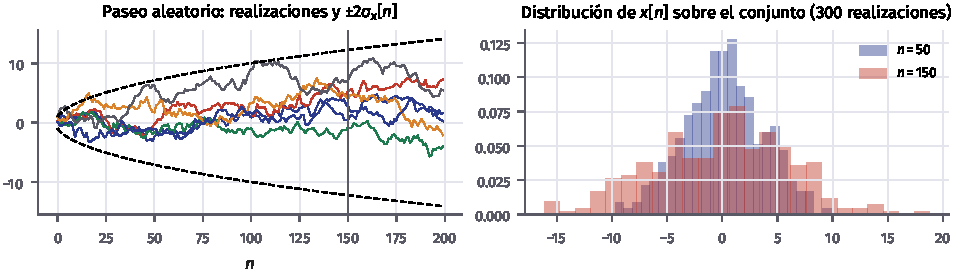
\includegraphics[width=0.74\linewidth]{realizaciones}\end{center}
  \footnotesize
  \begin{itemize}
    \item Fijado el resultado del experimento se obtiene una \alert{realización}, una señal determinista; fijado el instante $n$, $x[n]$ es una \alert{variable aleatoria}. El conjunto de todas las realizaciones es el \alert{conjunto} (\emph{ensemble}).
    \item En la figura, paseo aleatorio $x[n]=x[n-1]+w[n]$ con $w[n]\sim\mathcal N(0;0{,}25)$: la dispersión crece con $n$.
  \end{itemize}
\end{frame}

\begin{frame}{Cómo se describe}
  \footnotesize
  \begin{itemize}
    \item Completamente: con la distribución conjunta de $x[n_1],\dots,x[n_k]$ para cualesquiera instantes. Casi nunca se conoce.
    \item En la práctica, con los \alert{momentos de primer y segundo orden}:
  \end{itemize}
  \begin{definicion}[Estadísticos de una señal aleatoria]
    \begin{tabular}{@{}ll@{}}
      Media & $\mu_x[n]=E\{x[n]\}$\\[2pt]
      Valor cuadrático medio (potencia instantánea) & $E\{x^2[n]\}$\\[2pt]
      Autocorrelación & $\phi_{xx}[n_1,n_2]=E\{x[n_1]\,x[n_2]\}$\\[2pt]
      Autocovarianza & $\gamma_{xx}[n_1,n_2]=\phi_{xx}[n_1,n_2]-\mu_x[n_1]\mu_x[n_2]$\\[2pt]
      Correlación cruzada de $x$ e $y$ & $\phi_{xy}[n_1,n_2]=E\{x[n_1]\,y[n_2]\}$
    \end{tabular}
  \end{definicion}
  \begin{itemize}
    \item Son los estadísticos de la parte~2 aplicados a las variables $x[n_1]$ y $x[n_2]$. En continuo, igual con $x(t_1)$ y $x(t_2)$.
    \item Si la señal es \alert{gaussiana} (toda conjunta es gaussiana), media y autocorrelación la describen por completo.
  \end{itemize}
\end{frame}

\begin{frame}{Algunos tipos de señales aleatorias}
  \small
  \begin{itemize}
    \item \alert{Independiente e idénticamente distribuida} (i.i.d.): todas las $x[n]$ independientes y con la misma distribución. Con media nula es \alert{ruido blanco}.
    \item \alert{De Markov} (de primer orden): $x[n]$ solo depende del pasado a través de $x[n-1]$:
    \[
      f(x[n]\,|\,x[n-1],x[n-2],\dots)=f(x[n]\,|\,x[n-1]),
    \]
    y la conjunta se factoriza: $f(x[0],\dots,x[n])=f(x[0])\prod_{k=1}^nf(x[k]\,|\,x[k-1])$.
    \begin{itemize}
      \item Paseo aleatorio: $x[n]=x[n-1]+w[n]$, con $w$ ruido blanco.
      \item Autorregresiva de orden 1, AR(1): $x[n]=a\,x[n-1]+w[n]$, $\abs a<1$. Es ruido blanco filtrado por $1/(1-az^{-1})$.
    \end{itemize}
    \item En continuo, el papel del retardo lo hace la derivada: una señal de Markov continua cumple $\dv{x}{t}=-\alpha x(t)+w(t)$.
  \end{itemize}
  \nota{Las transparencias antiguas factorizaban la Markov sin el término $f(x[0])$ y escribían $p(\dot x(t)|x(t))$ sin decir de qué modelo salía.}
\end{frame}

% =====================================================================
\section{Estacionariedad y ergodicidad}

\begin{frame}{Estacionariedad}
  \small
  \begin{itemize}
    \item \alert{Estacionaria en sentido estricto}: ninguna distribución conjunta cambia al desplazar el origen de tiempos.
    \item \alert{Estacionaria en sentido amplio} (ESA): basta con los momentos de orden 1 y 2:
    \[
      \mu_x[n]=\mu_x\ \text{constante},\qquad\phi_{xx}[n+l,n]=\phi_{xx}[l]\ \text{solo depende de la separación }l.
    \]
    Entonces también $E\{x^2[n]\}=\phi_{xx}[0]$ y $\sigma_x^2$ son constantes.
    \item Dos señales son \alert{conjuntamente ESA} si cada una lo es y $\phi_{xy}[n+l,n]=\phi_{xy}[l]$.
  \end{itemize}
  \begin{definicion}[Notación para señales ESA]
    \[
      \phi_{xx}[l]=E\{x[n+l]\,x[n]\},\qquad\phi_{xy}[l]=E\{x[n+l]\,y[n]\},\qquad\gamma_{xx}[l]=\phi_{xx}[l]-\mu_x^2 .
    \]
    En continuo, $\phi_{xx}(\tau)=E\{x(t+\tau)\,x(t)\}$.
  \end{definicion}
  \nota{Errata antigua: se definía la estacionariedad en sentido amplio con $p(x(t_1))=p(x(t_2))$, que es una condición sobre toda la distribución de primer orden, ni necesaria ni suficiente para la ESA.}
\end{frame}

\begin{frame}{¿Cuáles son estacionarias?}
  \begin{center}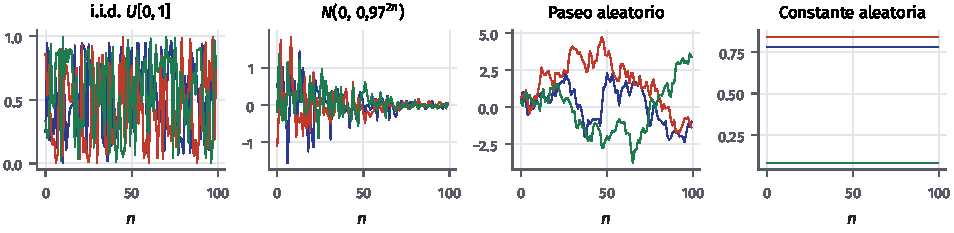
\includegraphics[width=\linewidth]{estacionariedad}\end{center}
  \footnotesize
  \begin{enumerate}
    \item i.i.d.\ $\mathcal U[0,1]$: \alert{sí}; misma distribución siempre y $\phi_{xx}[l]=\mu^2$ para $l\ne0$.
    \item Independientes $\mathcal N(0,\sigma^2[n])$ con varianza que cambia: \alert{no}; la varianza depende de $n$.
    \item Paseo aleatorio con $x[0]=0$: \alert{no}; $\operatorname{Var}\{x[n]\}=n\sigma_w^2$ crece.
    \item Constante aleatoria $x[n]=A$, $A\sim\mathcal U[0,1]$: \alert{sí}; $\mu_x=\frac12$ y $\phi_{xx}[l]=E\{A^2\}=\frac13$.
  \end{enumerate}
\end{frame}

\begin{frame}{Sinusoide de fase aleatoria}
  \begin{center}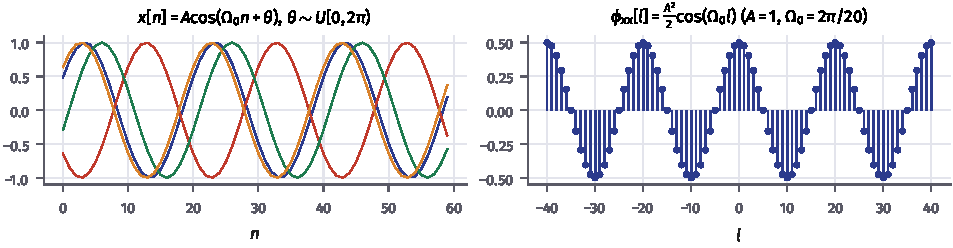
\includegraphics[width=0.9\linewidth]{fase_aleatoria}\end{center}
  \small
  Con $\theta\sim\mathcal U[0,2\pi)$:
  \(
    \mu_x=E\{A\cos(\Omega_0n+\theta)\}=0
  \)
  y
  \[
    \phi_{xx}[n+l,n]=\frac{A^2}2E\{\cos(\Omega_0(2n+l)+2\theta)+\cos(\Omega_0l)\}=\frac{A^2}2\cos(\Omega_0l).
  \]
  Es ESA. La autocorrelación de una componente periódica es periódica y no se amortigua.
\end{frame}

\begin{frame}{Ergodicidad}
  \small
  \begin{itemize}
    \item En la práctica solo se dispone de \alert{una} realización. ¿Se pueden obtener los estadísticos promediando en el tiempo en lugar de sobre el conjunto?
    \item Una señal ESA es \alert{ergódica} (en media y en autocorrelación) si
    \[
      \lim_{N\to\infty}\frac1{2N+1}\sum_{n=-N}^Nx[n]=\mu_x,\qquad
      \lim_{N\to\infty}\frac1{2N+1}\sum_{n=-N}^Nx[n+l]\,x[n]=\phi_{xx}[l]
    \]
    para casi todas las realizaciones. En continuo, igual con $\frac1{2T}\int_{-T}^T$.
    \item Ejemplos:
    \begin{itemize}
      \item i.i.d.\ y AR(1) estacionaria: ergódicas.
      \item Sinusoide de fase aleatoria: ergódica.
      \item Constante aleatoria: estacionaria pero \alert{no} ergódica; cada realización da su propia $A$, no $\frac12$.
      \item Las no estacionarias no se consideran ergódicas.
    \end{itemize}
  \end{itemize}
\end{frame}

% =====================================================================
\section{Autocorrelación}

\begin{frame}{Propiedades de la autocorrelación (señales ESA)}
  \small
  \begin{itemize}
    \item $\phi_{xx}[0]=E\{x^2[n]\}=\sigma_x^2+\mu_x^2$: la \alert{potencia} media.
    \item Par: $\phi_{xx}[-l]=\phi_{xx}[l]$.
    \item Máximo en el origen: $\abs{\phi_{xx}[l]}\le\phi_{xx}[0]$.
    \item Si no hay componentes periódicas ni constantes aleatorias, los valores alejados son incorrelados: $\gamma_{xx}[l]\to0$ y $\phi_{xx}[l]\to\mu_x^2$ cuando $\abs l\to\infty$.
  \end{itemize}
  \begin{importante}[¿Tiene la señal una componente determinista?]
    Si $\phi_{xx}[l]$ no tiende a $\mu_x^2$, sí; si la parte determinista es periódica, $\phi_{xx}$ oscila con el mismo periodo. Es un modo de detectar periodicidades enterradas en ruido.
  \end{importante}
  \nota{Erratas antiguas: «$\phi_{XX}(0)>\phi_{XX}(\tau)$» debe ser $\phi_{xx}(0)\ge\abs{\phi_{xx}(\tau)}$ (una sinusoide alcanza el máximo en cada periodo), y el límite es para $\abs\tau\to\infty$, no «para $t\gg0$».}
\end{frame}

\begin{frame}{Estimar la autocorrelación}
  \footnotesize
  Con una realización de $N$ muestras (señal ergódica):
  \[
    \hat\phi_{xx}[l]=\frac1{N-\abs l}\sum_{n=0}^{N-1-\abs l}x[n+\abs l]\,x[n]\quad\text{(insesgado)},\qquad
    \check\phi_{xx}[l]=\frac1N\sum_{n=0}^{N-1-\abs l}x[n+\abs l]\,x[n]\quad\text{(sesgado)}.
  \]
  \begin{itemize}
    \item El insesgado acierta en media, pero con $\abs l$ cerca de $N$ promedia pocos productos y es muy ruidoso. El sesgado se amortigua hacia los extremos y tiene menos varianza.
    \item Se usa solo hasta $\abs l$ bastante menor que $N$.
    \item Matlab: \texttt{xcorr(x, L, 'unbiased')} o \texttt{'biased'}; Python: \texttt{np.correlate(x, x, 'full')} dividido por el número de productos.
  \end{itemize}
\end{frame}

\begin{frame}{En código: autocorrelación de ruido i.i.d.}
  \codigo[basicstyle=\ttfamily\fontsize{6.6}{7.5}\selectfont]{autocorrelacion}
\end{frame}

\begin{frame}{Ejemplos}
  \begin{center}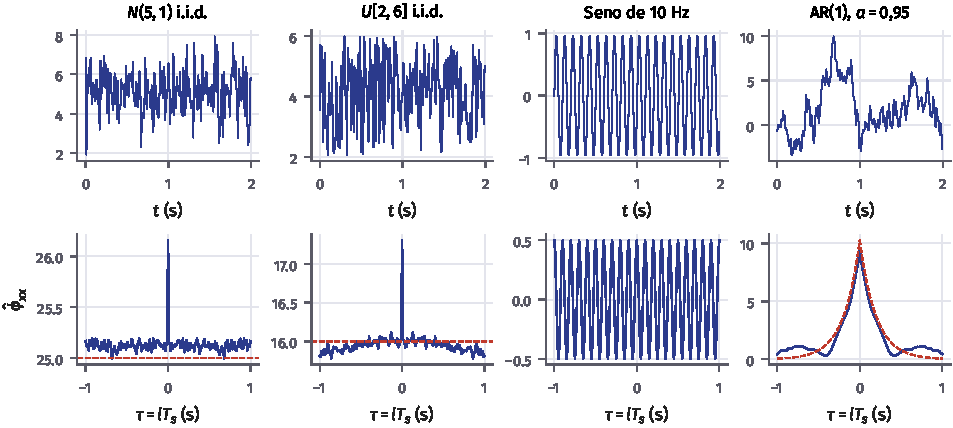
\includegraphics[width=0.84\linewidth]{autocorrelacion_ejemplos}\end{center}
  \footnotesize
  $T_s=0{,}01$\,s, 10\,s de señal. $\mathcal N(5,1)$: pico de $\sigma^2+\mu^2=26$ y $\mu^2=25$ fuera. $\mathcal U[2,6]$: $E\{X^2\}=\frac{52}3=17{,}3$ y $\mu^2=16$. El seno: oscila sin amortiguarse. AR(1): $\phi_{xx}[l]=\frac{a^{\abs l}}{1-a^2}\sigma_w^2$ (rojo).
\end{frame}

\begin{frame}{En código: AR(1)}
  \codigo{ar1}
  \nota{$x[n]=ax[n-1]+w[n]$ estacionaria: $\sigma_x^2=\sigma_w^2/(1-a^2)$ y $\phi_{xx}[l]=\sigma_x^2a^{\abs l}$. Con $a=0{,}9$, $\sigma_x^2=5{,}26$: el filtro amplifica el ruido.}
\end{frame}

% =====================================================================
\section{Correlación cruzada}

\begin{frame}{Correlación cruzada}
  \small
  \begin{itemize}
    \item $\phi_{xy}[l]=E\{x[n+l]\,y[n]\}$: cuánto se parece $x$ desplazada $l$ muestras a $y$.
    \item No tiene por qué tener el máximo en $l=0$ ni ser par: $\phi_{xy}[l]=\phi_{yx}[-l]$.
    \item Cotas: $\abs{\phi_{xy}[l]}^2\le\phi_{xx}[0]\,\phi_{yy}[0]$ y $\abs{\phi_{xy}[l]}\le\frac12\big(\phi_{xx}[0]+\phi_{yy}[0]\big)$.
    \item Si $x$ e $y$ son independientes, $\phi_{xy}[l]=\mu_x\mu_y$ para todo $l$.
  \end{itemize}
  \begin{ejemplo}[Eco]
    $y[n]=\alpha\,x[n-D]+v[n]$, con $x$ blanco de varianza $\sigma_x^2$ y $v$ independiente:
    \[
      \phi_{yx}[l]=E\{y[n+l]\,x[n]\}=\alpha\,\phi_{xx}[l-D]=\alpha\sigma_x^2\,\delta[l-D].
    \]
    El pico de la correlación cruzada está en el retardo $D$.
  \end{ejemplo}
  \nota{Convenio de Oppenheim y Schafer, y de \texttt{xcorr(x, y)} en Matlab. Otros textos (y la versión antigua) definen $E\{x(t)\,y(t+\tau)\}$, que es la misma función reflejada.}
\end{frame}

\begin{frame}{Aplicación: medir un retardo}
  \begin{center}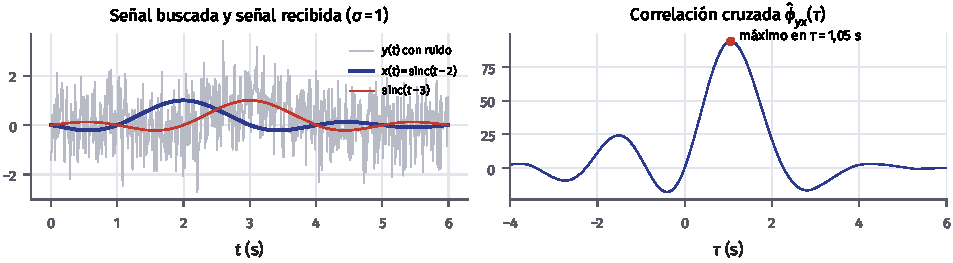
\includegraphics[width=0.68\linewidth]{retardo}\end{center}
  \codigo[basicstyle=\ttfamily\fontsize{6.3}{7}\selectfont]{retardo}
\end{frame}

\begin{frame}{Otras aplicaciones}
  \begin{itemize}
    \item \alert{Radar y sonar}: se emite un pulso conocido y se correla el eco recibido con él (filtro adaptado); el retardo da la distancia.
    \item \alert{Localización}: con dos micrófonos, el retardo entre sus señales da la dirección de la fuente.
    \item \alert{Caminos múltiples}: un pico por cada camino de propagación.
    \item \alert{Sincronización}: encontrar el inicio de una trama en comunicaciones (GPS, Wi-Fi).
    \item \alert{Identificación de sistemas}: con entrada blanca, $\phi_{yx}[l]=\sigma_x^2h[l]$ (parte~4).
  \end{itemize}
\end{frame}

% =====================================================================
\section*{Resumen}
\begin{frame}{Conceptos importantes}
  \begin{columns}[T]
    \begin{column}{0.5\textwidth}
      \begin{itemize}
        \item Señal aleatoria: variables indexadas por $n$; realizaciones y conjunto.
        \item $\mu_x[n]$, $\phi_{xx}[n_1,n_2]$, $\gamma_{xx}$, $\phi_{xy}$.
        \item ESA: media constante, $\phi_{xx}[l]=E\{x[n+l]x[n]\}$.
        \item Ergódica: promedios temporales = de conjunto.
      \end{itemize}
    \end{column}
    \begin{column}{0.5\textwidth}
      \begin{itemize}
        \item $\phi_{xx}[0]$ potencia; par; $\abs{\phi_{xx}[l]}\le\phi_{xx}[0]$; $\to\mu_x^2$.
        \item Estimadores sesgado e insesgado (\texttt{xcorr}).
        \item Correlación cruzada: retardos y ecos.
      \end{itemize}
    \end{column}
  \end{columns}
  \bigskip
  \gris{Apuntes del Tema 6, sección 3 · Hoja de ejercicios, ejercicios 11–14.}
\end{frame}

\end{document}
